\begin{figure}[tb]
  \centering
  \begin{subfigure}[b]{0.32\textwidth}
    
\includegraphics[width=\textwidth]{./img/raw/cs-opdeling-voorbeeld/render.png}
    \caption{De gerenderde afbeelding.}
    \label{fig:cs-opdeling-voorbeeld:render}
  \end{subfigure}%
  \begin{subfigure}[b]{0.32\textwidth}
    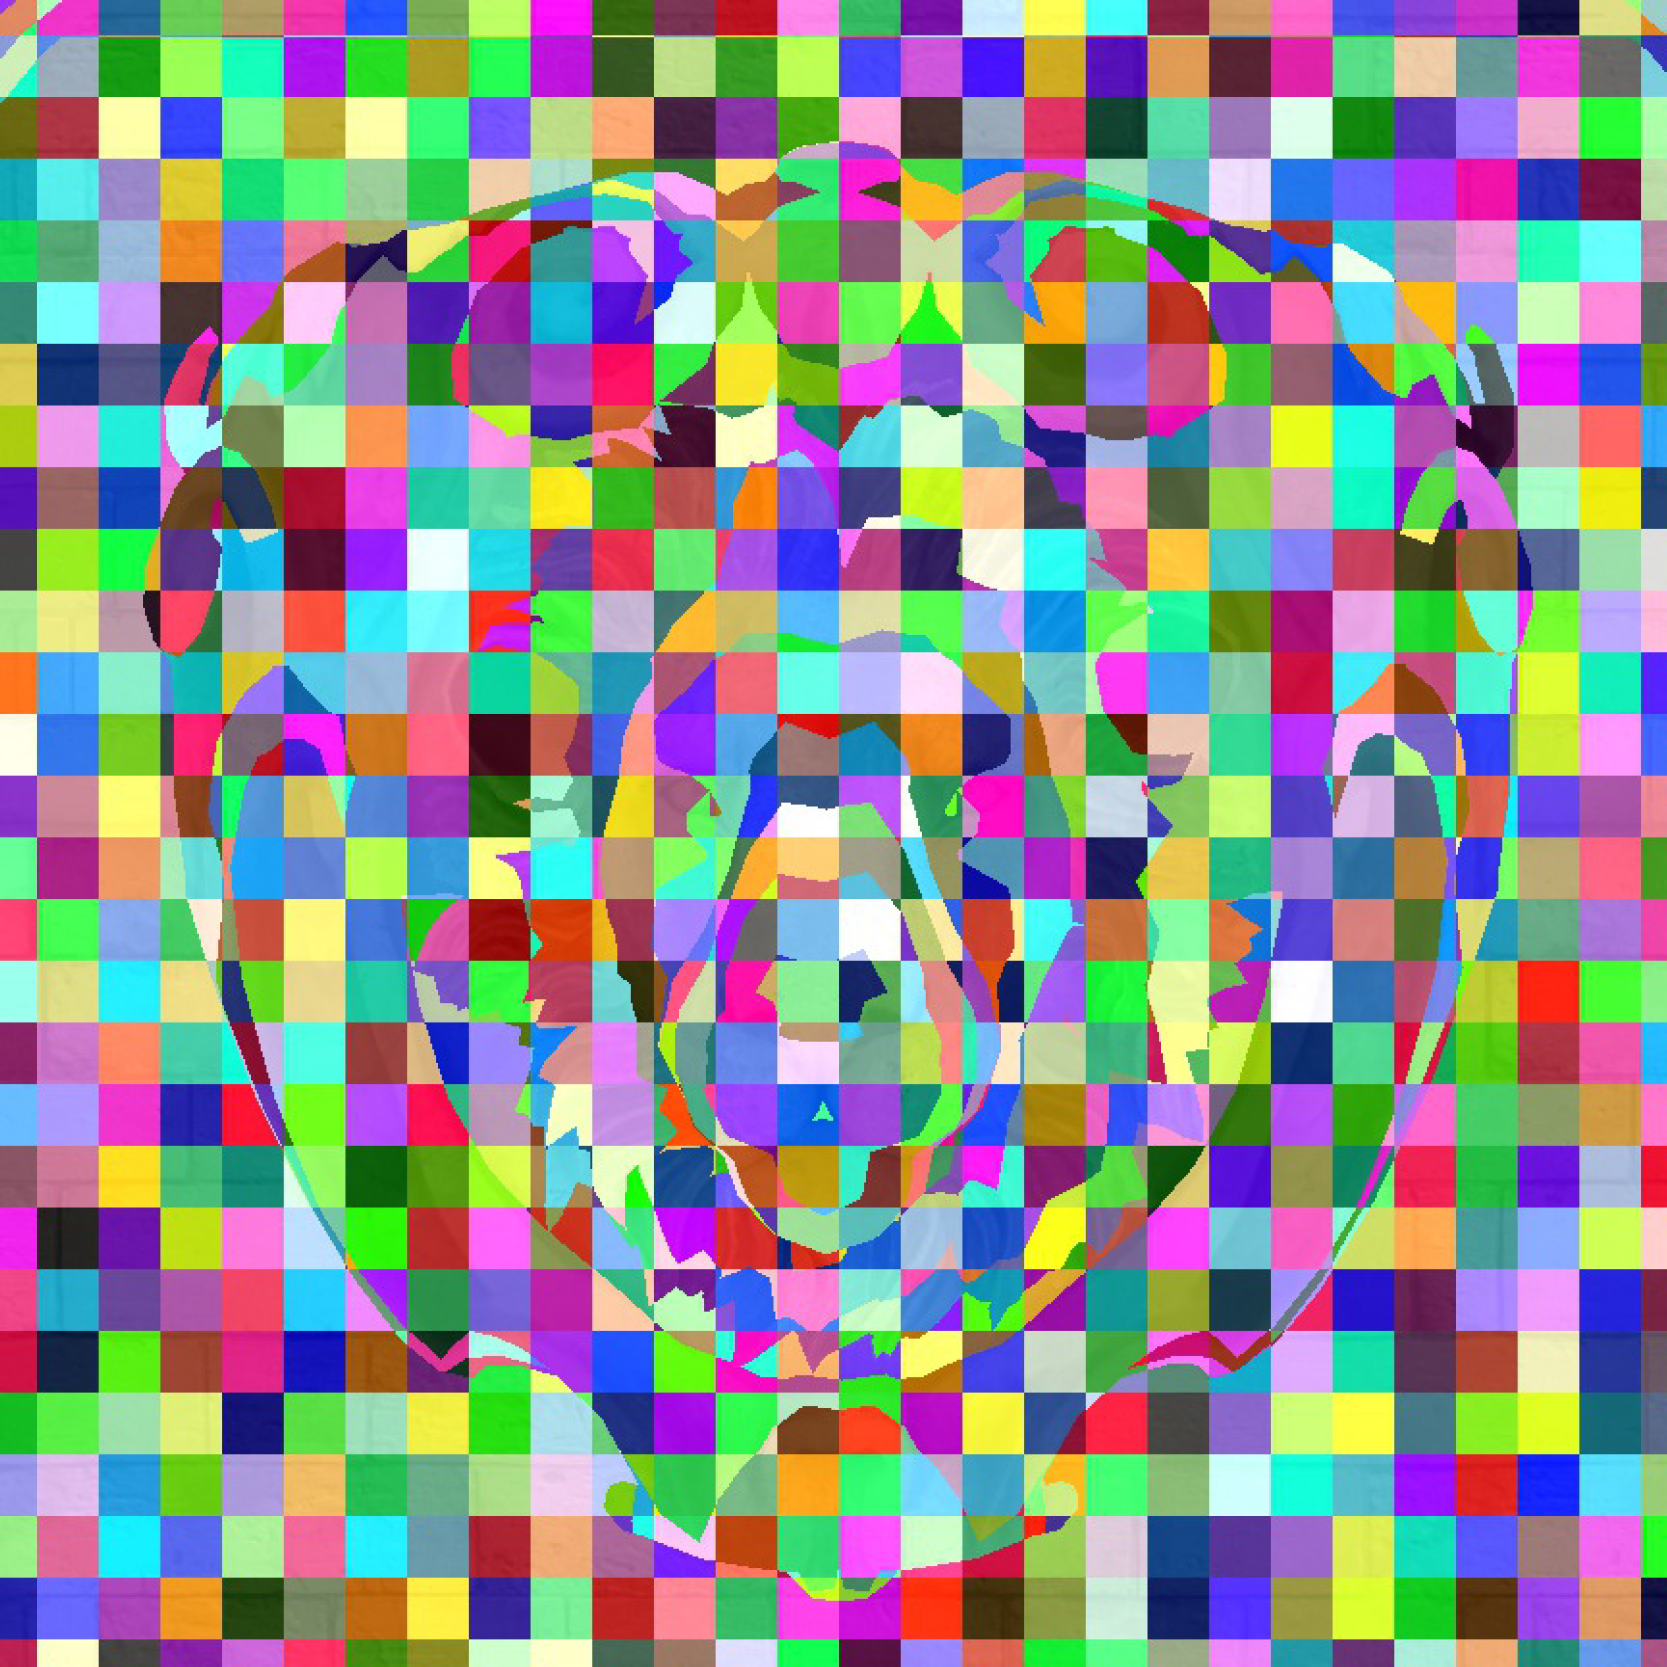
\includegraphics[width=\textwidth]{./img/raw/cs-opdeling-voorbeeld/depth.png}
    \caption{Op basis van diepte.}
    \label{fig:cs-opdeling-voorbeeld:depth}
  \end{subfigure}%
  \begin{subfigure}[b]{0.32\textwidth}
    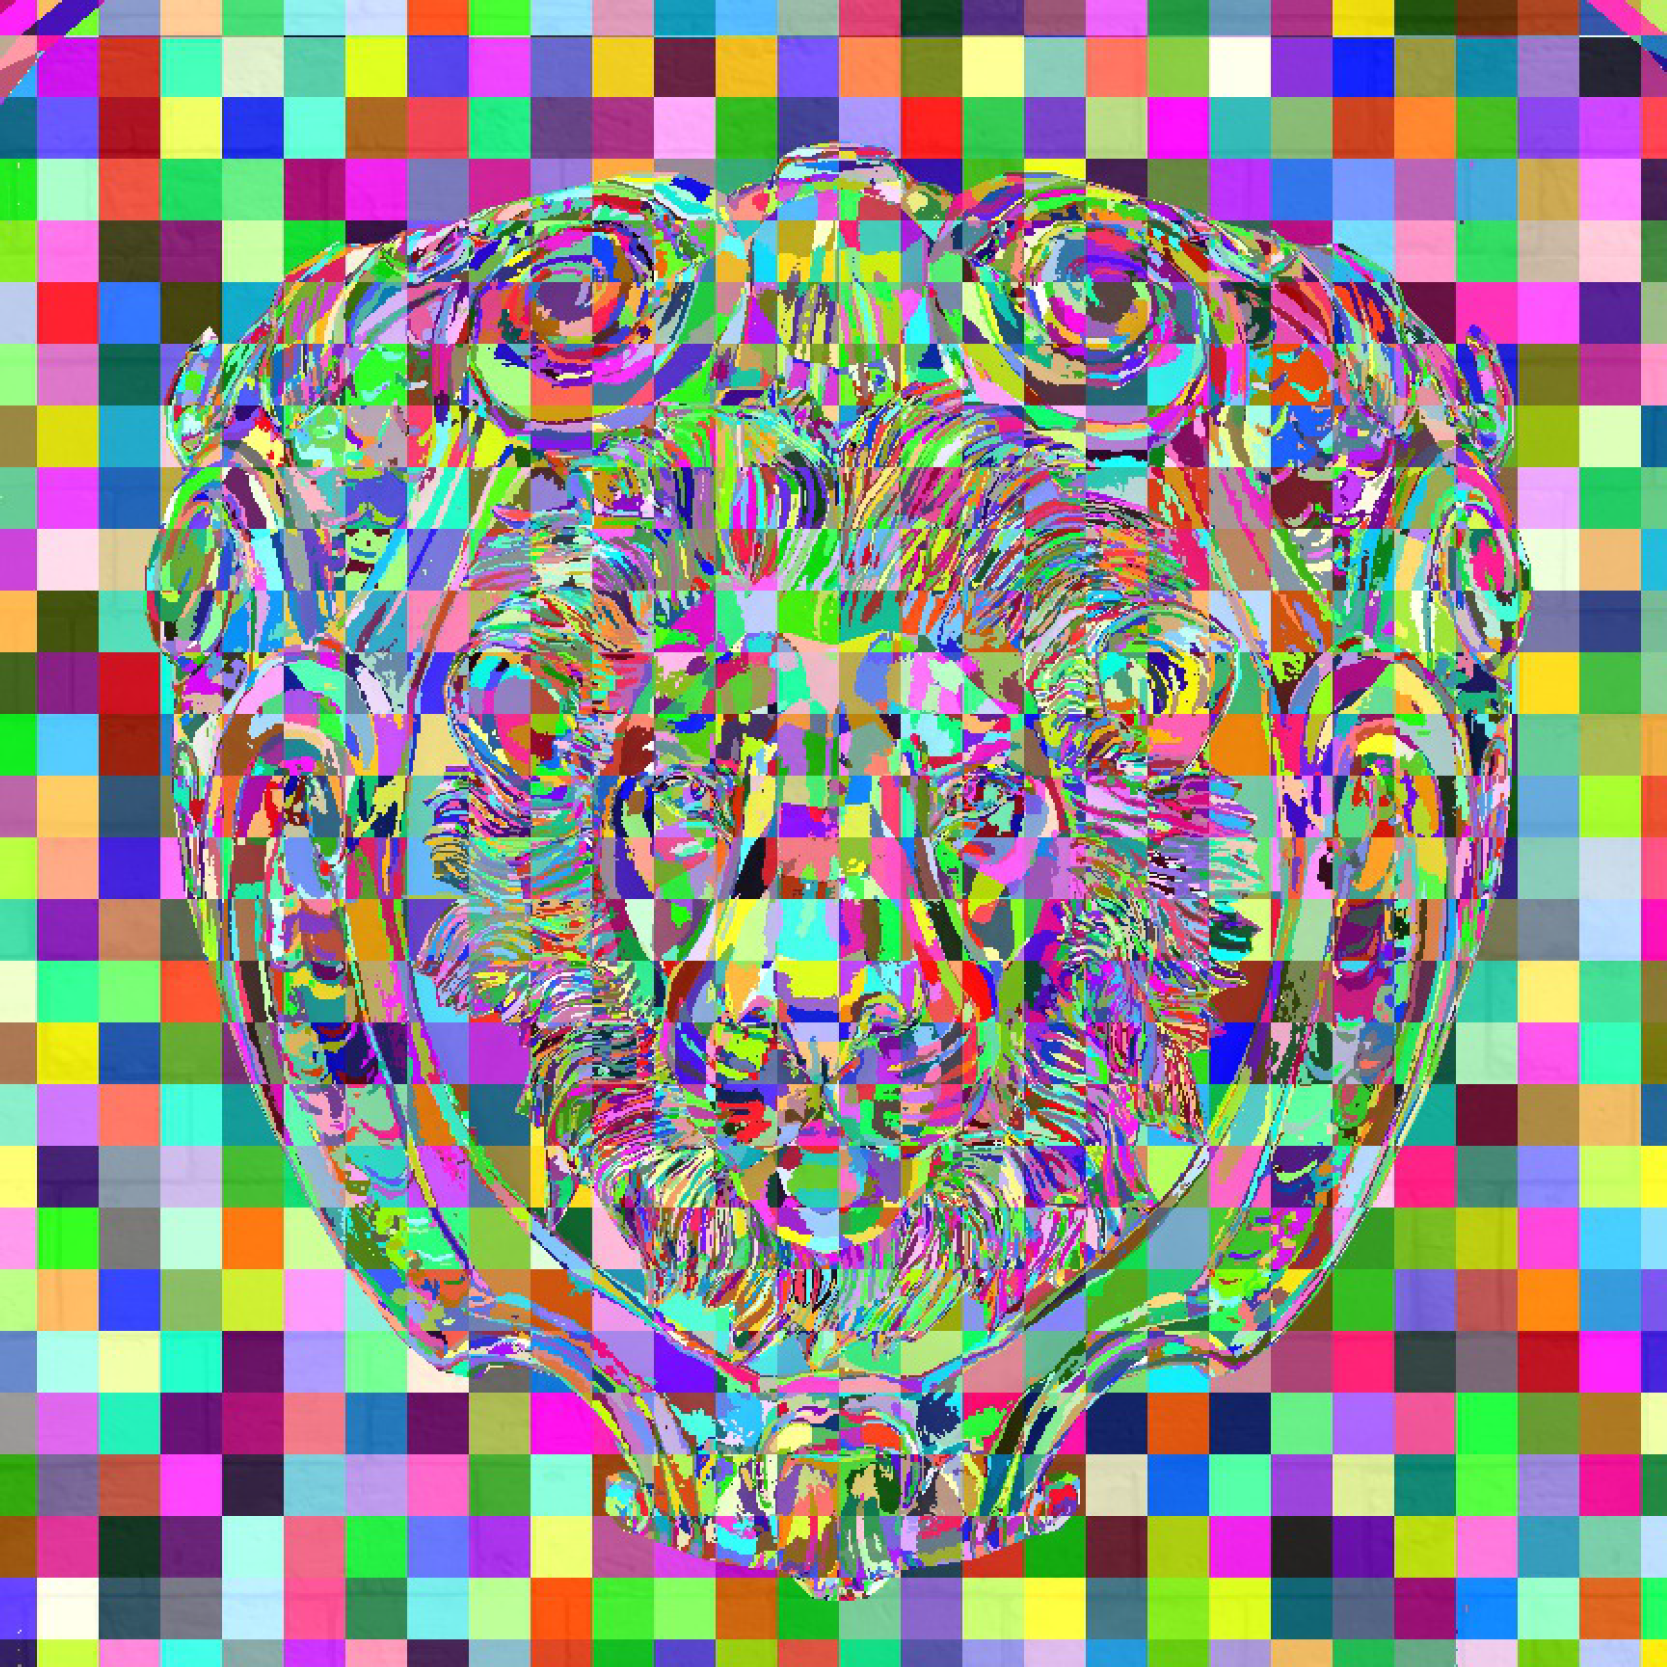
\includegraphics[width=\textwidth]{./img/raw/cs-opdeling-voorbeeld/normal.png}
    \caption{Op basis van normaal.}
    \label{fig:cs-opdeling-voorbeeld:normaal}
  \end{subfigure}
  \caption{Clustering op basis van diepte, en diepte en normaal.}
  \label{fig:cs-opdeling-voorbeeld}
\end{figure}
